\section{Utterance Embeddings}\label{sec:utt2vec}
\roger{This section still contains some redundant parts and needs to be restructured.}
Neural networks for distributional semantics has gained relevant importance in the past years since the publication of the first neural network word embedding models. One of the main reasons for that was the discovery that dense high-dimensional vector representations of words are able to capture semantic relations between words \cite{mikolov2013efficient}.  Figure~\ref{fig:w2v_example} shows a typical example where simple vector addition and subtraction lead to analogies such that the vector difference between \textit{woman} and \textit{man} is the same as between \textit{aunt} and \textit{uncle}, for example.


\begin{figure}
\centering
\begin{minipage}{.4\textwidth}
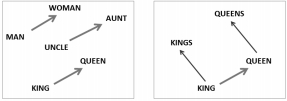
\includegraphics[width=1\textwidth]{img/w2v_example}
\caption{Word2vec semantic relations.}
\label{fig:w2v_example}
\end{minipage}
\end{figure}

In distributional semantic models, word embeddings are learned by predicting words within a context of other words. Base don the fact that similar words occur in similar contexts, these models are capable of successfully representing words in high-dimensional vectors.

This approach is no longer feasible on a sentence level, as the vocabulary of all observed sentences is larger than the word-based vocabulary leading to sparse contexts. Therefore, a slightly different neural network approach for learning representations for sentences has been proposed by Le and Mikolov \shortcite{le2014distributed}, in which sentence vectors are learned from the words within the sentences.  In this case, sentence embeddings are trained together with word embeddings. The latter are shared for the entire model.

This model makes it possible to map word sequences of any length to vectors of fixed dimensionality. Moreover, its unsupervised nature allows any raw corpus to be used for training.

\david{as the paragraphs above might be the complicated part of our research we should spend some time getting this as clear and readable as possible}

\roger{The part below should be merged with the part above.}
\subsection{Utterance embeddings} 

In order to get vector representations from utterances, we use an extension of the word embeddings neural network proposed by Mikolov\cite{mikolov2013efficient}. Originally, these networks had two main architectures, know as \emph{Continuous-bag-of-words} and \emph{Skip-gram}. In the first case, they were optimized so as to predict the next word given its context, while in the latter, a word is input and the context is predicted. Due to word co-occurrences, these models are able to effectively capture the meaning of the words. The co-occurrence property present at the word level is no longer valid when handling phrases. For sentence embeddings a novel approach was recently introduced \lau{cite}, in which a similar training algorithm is followed. In this case, two structures are maintained (one for words, and one for sentence representations); the word structure is shared across all sentences, while the sentence structure is only valid for the current paragraph. The task is the same as before: given a certain window, the model is optimized to predict the missing word; but this time, the context representation is constructed using the individual word vectors as well as the paragraph vector. This training schema is called \emph{Paragraph Vector Distributed memory (PV-DM)}, and it is the one we use to train our model. Figure~\ref{fig:p2v_arq} shows the \emph{PV-DM} architecture.

\begin{figure}
\centering
\begin{minipage}{.3\textwidth}
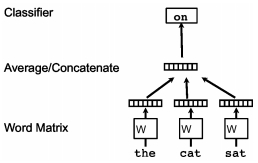
\includegraphics[width=1\textwidth]{img/par2vec_arq}
\caption{Paragraph vector PV-DM architecture.}
\label{fig:p2v_arq}
\end{minipage}
\end{figure}

Once the model is trained, it can be queried so as to get the vector representations for each already seen sentence. It can also be used to \emph{infer} vector mappings of \emph{unseen} sentences. This second step will be crucial to get representations for utterances in our test dataset.

A great advantage of these approach is that it is completely unsupervised, and thus, we can use any amount of unlabelled data we want.

\subsubsection*{Word2vec pretrained vectors}
The implementation we use for getting paragraph vectors allows us to use already trained word embeddings. The way in which this feature works follows can be summarized as: (a) No new words are added to the vocabulary; (b) Intersecting words adopt pretrained values ; (c) Non intersecting words are left alone.
For our experiments, we try both alternatives, training word and paragraph embeddings from scratch using several dialog corpora as input, and also using freely available embeddings\footnote{\url{https://code.google.com/p/word2vec/}}.